\documentclass[../main/main.tex]{subfiles}

\raggedbottom

\makeatletter
\renewcommand{\@chapapp}{M\'ecanique -- chapitre}
\makeatother

% \toggletrue{student}

\begin{document}
\setcounter{chapter}{5}

\chapter{Moment cin\'etique pour un point mat\'eriel}
Jusqu'à présent, nous avons vu deux méthodes de résolution en mécanique~:
\begin{itemize}
    \item Le PFD au chapitre 1, pour avoir toute l'information sur un
        mouvement~;
    \item Les théorèmes énergétiques (TEC et TEM, TPC et TPM) au chapitre 4,
        pour les informations à un instant donné.
\end{itemize}
Il existe une autre méthode de résolution dans le cas spécifiques des
\textbf{mouvements de rotation}~: le théorème du moment cinétique. Dans ce
chapitre, \textbf{nous ne nous intéressons qu'à des points matériels M} de masse
$m$~: le traitement des solides viendra un peu plus tard.

\section{Moment d'une force}
\subsection{Par rapport à un point}
\textbf{Observations}~:
\begin{itemize}
    \item Lorsqu'une masse $m$ est placée à distance d'un point «~pivot~», cette
        masse génère une rotation.
    \item On peut compenser cette rotation en mettant une même masse à la même
        distance de l'autre côté.
    \item On peut compenser une masse plus grande en mettant une masse plus
        faible plus loin du pivot.
    \item Ainsi l'effet est proportionnel à la distance au pivot.
\end{itemize}

\begin{minipage}{0.45\linewidth}
    \begin{center}
        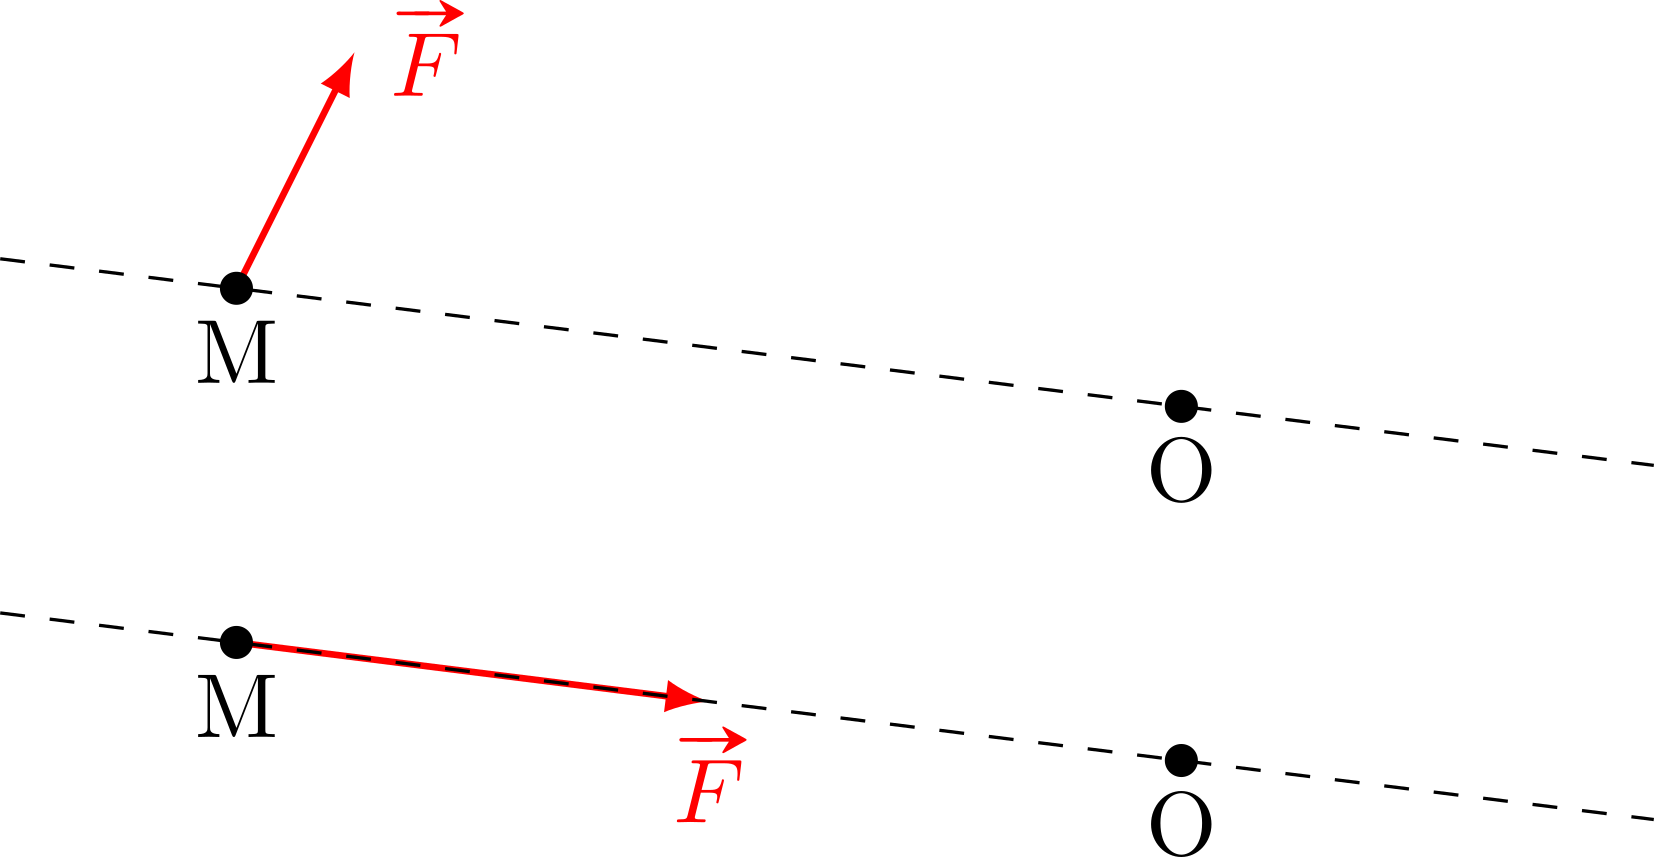
\includegraphics[scale=1]{moment_intro}
    \end{center}
\end{minipage}
\hfill
\begin{minipage}{0.45\linewidth}
    $\Ff$ tend à faire tourner M autour de O dans le sens horaire.\\[2.5em]
    $\Ff$ ne cause aucune rotation.
\end{minipage} \bigbreak

Pour traduire cette capacité d'une force à créer un mouvement de rotation autour
de O, on introduit une grandeur appelée \textbf{moment d'une force}.

\begin{tdefi}{Définition~: moment d'une force, heart}
    Le moment d'une force $\Ff$ au point M par rapport à un point O est le
    \textbf{vecteur}~:
    \[\boxed{\Mcf_{\Or}(\Ff) = \OM\wedge\Ff}\quad\text{Unité~:~}\si{N.m}\]
    avec $\wedge$ le produit vectoriel.
\end{tdefi}

\textbf{Interprétation géométrique}~: la \textbf{direction} de
$\Mcf_{\Or}(\Ff)$ indique la manière dont la force $\Ff$ a tendance à faire
tourner M autour de O, et est donné par la \textbf{règle de la main droite}.
\begin{center}
    \begin{tabularx}{\linewidth}{YYY}
        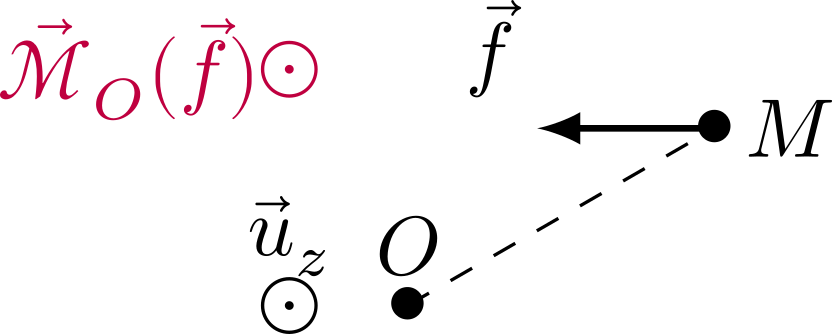
\includegraphics[scale=1]{moment_force-a} &
        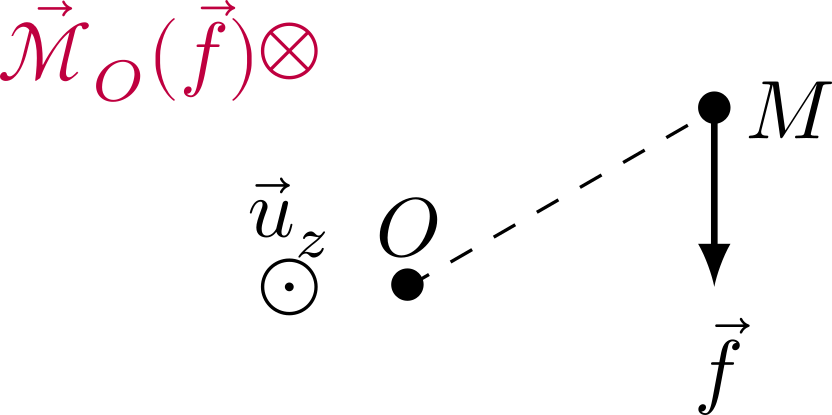
\includegraphics[scale=1]{moment_force-b} &
        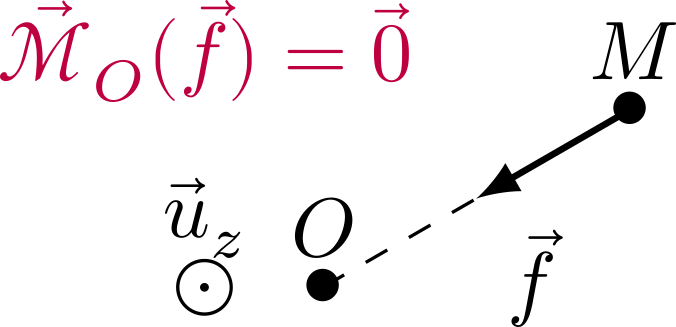
\includegraphics[scale=1]{moment_force-c}
        \\
        Si $\Mcf_{\Or}(\Ff)$ est dirigé selon $+\uz$, $\Ff$ fait tourner M dans
        le sens \textbf{direct}. &
        Si $\Mcf_{\Or}(\Ff)$ est dirigé selon $-\uz$, $\Ff$ fait tourner M dans
        le sens \textbf{horaire}. &
        Si $\Mcf_{\Or}(\Ff) = \of$, $\Ff$ ne fait pas tourner M autour du point
        O.
    \end{tabularx}
\end{center}

\begin{rexem}{Exercice}
    \begin{minipage}[c]{0.70\linewidth}
        Un véhicule assimilé à un point matériel M de masse $m$ se déplace de
        haut en bas d’une colline~; la trajectoire est assimilée à un quart de
        cercle vertical de centre O et de rayon $R$. On note $\tt$ l’angle que
        fait OM avec la verticale. Calculer le moment du poids par rapport à O.
    \end{minipage}
    \hfill
    \begin{minipage}{0.25\linewidth}
        \begin{center}
            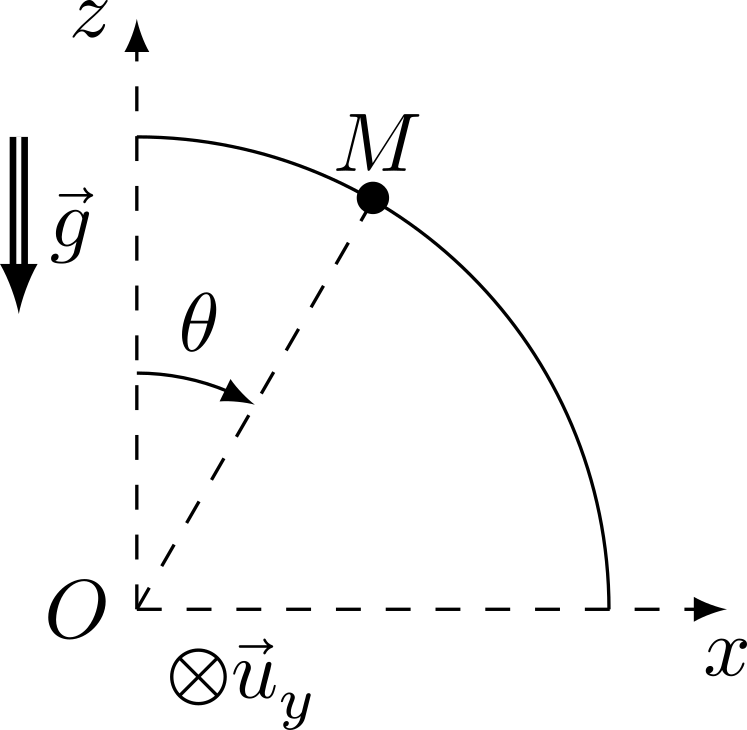
\includegraphics[scale=1]{moment_force-ex}
        \end{center}
    \end{minipage}
    \tcblower
    Pour calculer le moment d'une force, on décompose ladite force et le vecteur
    $\OM$ \textbf{dans la même base}. Ici, le poids s'exprime en coordonnées
    cartésiennes~: on projette donc la position $\OM$ dans le repère cartésien.
    On obtient ainsi~:
    \begin{gather*}
        \left\{
            \begin{aligned}
                \Pf &= -mg\uz\\
                \OM &= R\ur\\
                    &= R(\cos\tt\uz + \sin\tt\ux)
            \end{aligned}
        \right.
    \end{gather*}
    On peut donc calculer le moment du poids~:
    \begin{align*}
        \Mcf_{\Or}(\Pf) &= \OM\wedge\Pf\\
                        &= -mgR(\cos\tt\uz + \sin\tt\ux)\wedge\uz\\
                        &= -mgR\cos\tt\underbracket[1pt]{\uz\wedge\uz}_{=\of}
                           -mgR\sin\tt\underbracket[1pt]{\ux\wedge\uz}_{=-\uy}\\
        \Lra
        \Aboxed{
            \Mcf_{\Or}(\Pf) &= +mgR\sin\tt\uy
        }
    \end{align*}
    On vérifie \textbf{systématiquement} que la direction du moment donne bien
    le sens de rotation attendu, ici dans le horaire sur la figure.
\end{rexem}

\subsection{Par rapport à un axe \ul{orienté}}
Plutôt que de travailler avec des vecteurs, on peut simplement s'intéresser à la
norme d'un moment. On définit pour ça~:
\begin{tdefi}{Définition~: moment d'une force par rapport à un axe orienté,
    heart}
    Le moment d'une force par rapport à un axe orienté $(\Or,\uz)$ est le
    \textbf{scalaire} défini par~:
    \[\Mc_z(\Ff) = \left(\OM\wedge\Ff\right)\cdot\uz = \Mcf_{\Or}(\Ff)\cdot\uz\]
    avec O un point de l'axe $z$. $\Mc_z$ est donc le projeté du moment
    $\Mcf_{\Or}(\Ff)$ sur l'axe $(\Or z)$.
\end{tdefi}
\begin{rimpo}{Important}
    \begin{enumerate}
        \item $\Mc_z$ est un \textbf{scalaire} puisqu'il est issu d'un
            \textbf{produit scalaire}.
        \item $\Mc_z$ ne dépend pas du point O considéré.
    \end{enumerate}
\end{rimpo}
\textbf{Interprétation géométrique}~: cette fois-ci c'est le \textbf{signe} de
$\Mc_z$ qui indique le sens de rotation par rapport à l'axe orienté~: il est
positif si la rotation se fait dans le sens \textbf{direct}.

\subsection{Bras de levier d'une force}
Pour calculer le moment d'une force $\Ff$ exercée en un point M par rapport à un
axe orienté $\D$ (souvent $(\Or,\uz)$), on décompose $\Ff$ en deux composantes~:
l'une parallèle et l'une perpendiculaire à l'axe $\D$, notées $\Ff = \Ff_{\perp}
+ \Ff_{\parr}$. \smallbreak
\begin{center}
    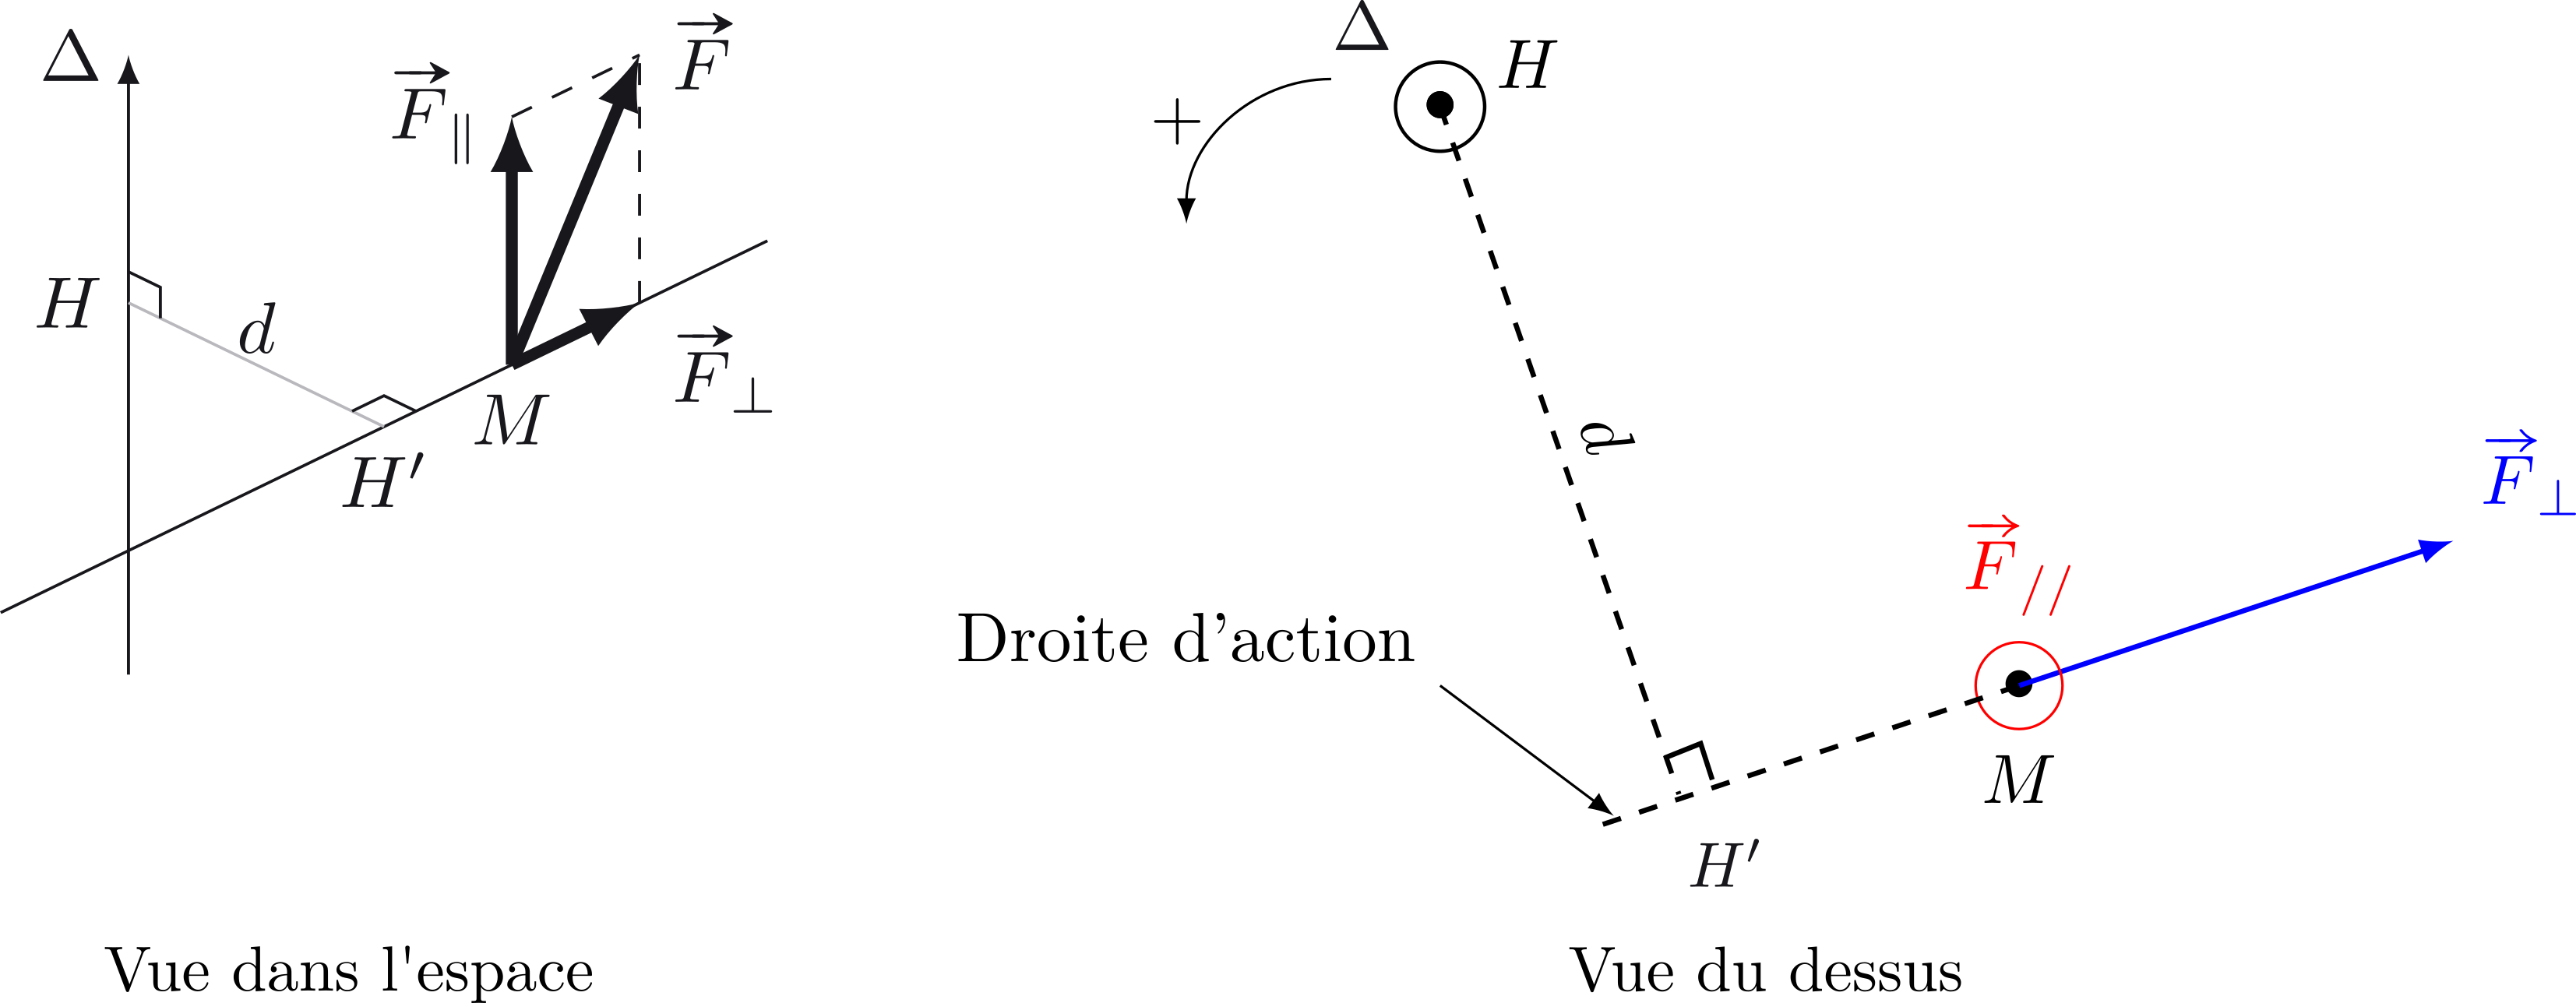
\includegraphics[scale=1]{bras_levier}
\end{center}
\begin{tprop}{Propriété~: bras de levier d'une force, heart}
    Le \textbf{bras de levier} d'une force $\Ff$ appliquée en un point M est la
    \textbf{distance $d$} entre l'\textbf{axe} de rotation et la \textbf{droite
    d'action} donnée par sa composante $\Ff_{\perp}$. Le moment $\Mc_z(\Ff)$ est
    alors
    \[\boxed{\Mc_z(\Ff) = \pm d\norm{\Ff_{\perp}}}\]
    On détermine le signe en regardant dans quelle direction la force
    $\Ff_{\perp}$ tend à faire tourner M.
\end{tprop}
\begin{tdemo}{Démonstration, hand}
    On commence par déterminer le moment de la force par rapport au point H de
    l'axe, puis on projettera par produit scalaire avec $\uz$. On a donc~:
    \begin{gather*}
        \vv{\rm HM} = \vv{\rm HH'} + \vv{\rm H'M}\\
        \Ff = \Ff_{\perp} + \Ff_{\parr}
    \end{gather*}
    Ainsi,
    \begin{align*}
        \Mcf_{\rm H}(\Ff) &= \vv{\rm HM}\wedge\Ff\\
                          &=
                          (\vv{\rm HH'} + \vv{\rm H'M})
                          \wedge
                          (\Ff_{\perp} + \Ff_{\parr})\\
                          &=
                          \underbracket[1pt]{
                              \vphantom{
                                  \underbracket[1pt]{\strut\vv{\rm H'M}}_
                                  {\parr\Ff_\perp}
                                  \wedge
                                  \Ff_{\perp}
                              }
                             \underbracket[1pt]{\strut\vv{\rm HH'}}_{\perp\uz}
                             \wedge
                             \underbracket[1pt]{\strut\Ff_{\perp}}_{\perp\uz}
                          }_{=\pm dF\uz} +
                          \underbracket[1pt]{
                              \vphantom{
                                  \underbracket[1pt]{\strut\vv{\rm H'M}}_
                                  {\parr\Ff_\perp}
                                  \wedge
                                  \Ff_{\perp}
                              }
                              \underbracket[1pt]{\strut\vv{\rm HH'}}_{\perp\uz}
                              \wedge
                              \underbracket[1pt]{\strut\Ff_{\parr}}_{\parr\uz}
                          }_{\perp\uz}+
                          \underbracket[1pt]{
                              \underbracket[1pt]{\strut\vv{\rm H'M}}_{\parr\Ff_\perp}
                              \wedge
                              \Ff_{\perp}
                          }_{=\of}+
                          \underbracket[1pt]{
                              \vphantom{
                                  \underbracket[1pt]{\strut\vv{\rm H'M}}_
                                  {\parr\Ff_\perp}
                                  \wedge
                                  \Ff_{\perp}
                              }
                              \underbracket[1pt]{\strut\vv{\rm H'M}}_{\perp\uz}
                              \wedge
                              \underbracket[1pt]{\strut\Ff_{\parr}}_{\parr\uz}
                          }_{\perp\uz}
        \shortintertext{Or,}
        \Mc_z(\Ff) &= \Mcf_{\rm H}(\Ff)\cdot\uz\\
        \Lra
        \Mc_z(\Ff) &= \pm dF_{\perp} + 0 + 0 + 0
        \qed
    \end{align*}
\end{tdemo}

En général, on s'intéressera directement à une force perpendiculaire à l'axe
orienté, auquel cas la situation se résume ainsi~:
\begin{figure}[H]
    \centering
    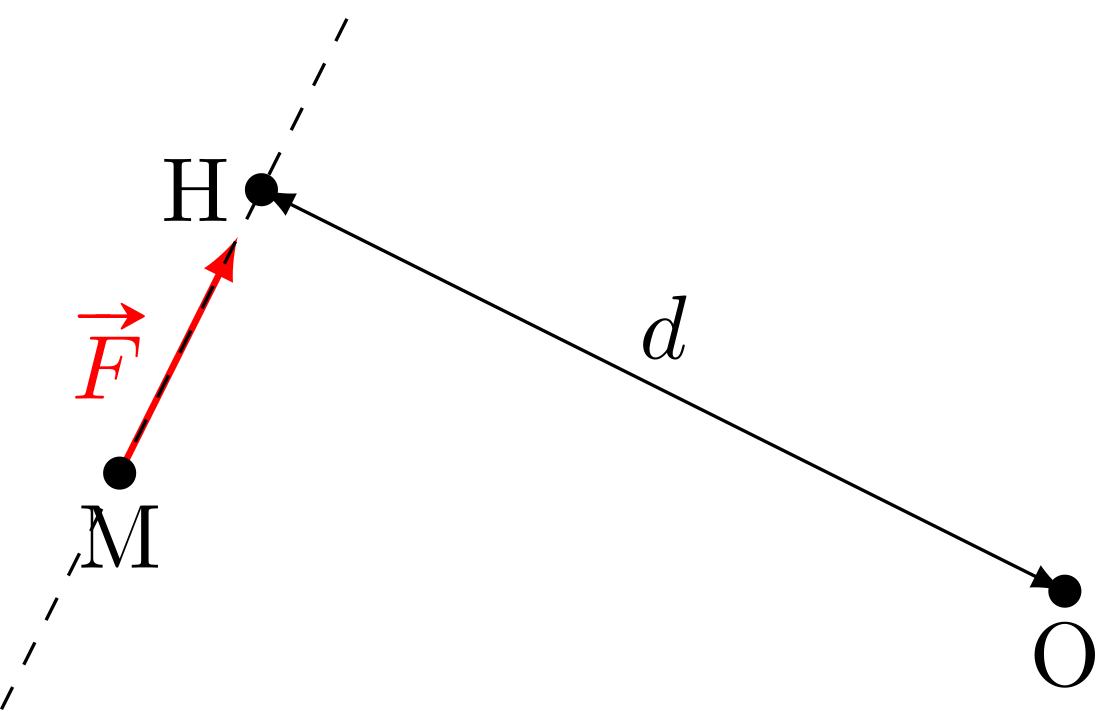
\includegraphics[scale=1]{bras_levier-simple}
\end{figure}
et on a alors
\[
    \OM\wedge\Ff =
        \underbracket[1pt]{\vv{\rm OH}\wedge\Ff}_{=\pm dF\uz} +
        \underbracket[1pt]{\vv{\rm HM}\wedge\Ff}_{=\of}
\]
On peut résumer ceci à la méthode suivante~:

\begin{tror}{Méthode du bras de levier, heart}
    \begin{enumerate}
        \item Trouver le point O de l'axe de rotation dans le plan
            perpendiculaire à $\uz$ passant par M~;
        \item Tracer la droite d'action, passant par M et dirigée par $\Ff$~;
        \item Calculer géométriquement $\Ff_\perp$ si nécessaire~;
        \item Calculer géométriquement $d$~;
        \item Identifier le sens de rotation avec la règle de la main droite.
    \end{enumerate}
\end{tror}

\begin{rexemside}{Exercice}
    On considère trois forces, de normes égales, exercées sur une porte pour
    l'ouvrir. Laquelle est la plus efficace~? Justifier à l'aide du bras de
    levier.
    \smallbreak
    \hdashrule[0.5ex]{1.1\linewidth}{.5pt}{3pt}
    \smallbreak
    \begin{enumerate}
        \item La première force créé un moment
            \[\Mc_z(\Ff_1) = d_1F\]
        \item La deuxième force créé un moment
            \[\Mc_z(\Ff_2) = d_2F > d_1F\]
        \item La troisième force créé un moment
            \[\Mc_z(\Ff_3) = d_2F_{3\perp} < d_2F\]
    \end{enumerate}
    \tcblower
    \begin{center}
        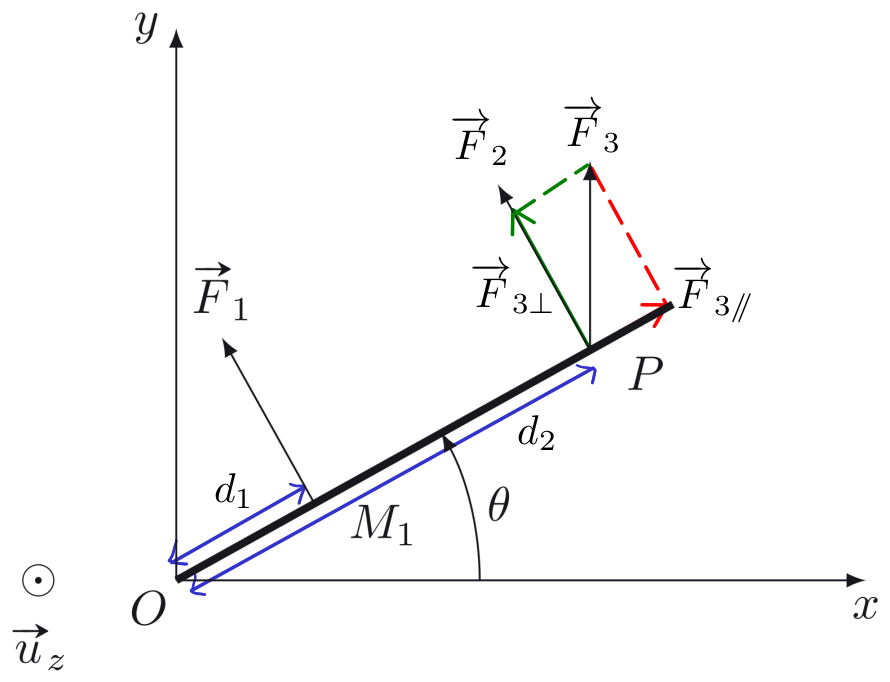
\includegraphics[width=\linewidth]{porte_right-corr}
        C'est donc $\Ff_2$ qui est la plus efficace.
    \end{center}
\end{rexemside}

\subsection{Exemples de calcul de moments}

\subsubsection{Clé sur un boulon}
\begin{minipage}[c]{0.25\linewidth}
    \begin{center}
        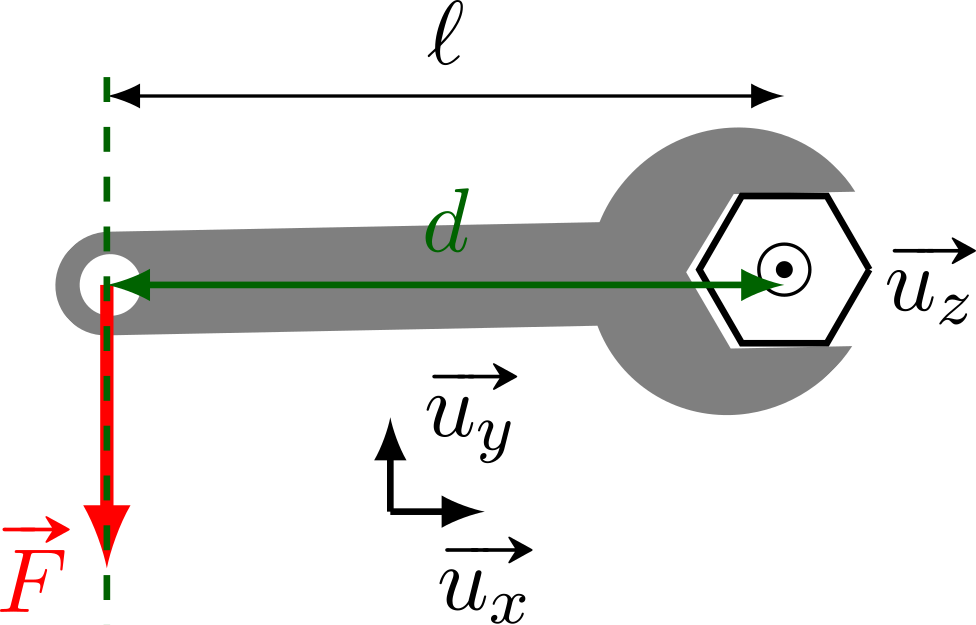
\includegraphics[scale=1]{moment_cle}
    \end{center}
\end{minipage}
\hfill
\begin{minipage}{0.70\linewidth}
    \begin{gather*}
        \Ff = -F\uy
        \qqet
        \OM = -\ell\ux
        \\
        \OM\wedge\Ff = \ell F\ux\wedge\uy = \ell F \uz
        \\
        \boxed{\Mc_z(\Ff) = \ell F}
    \end{gather*}
\end{minipage}

\subsubsection{Règle à l'horizontale}
\begin{minipage}[c]{0.25\linewidth}
    \begin{center}
        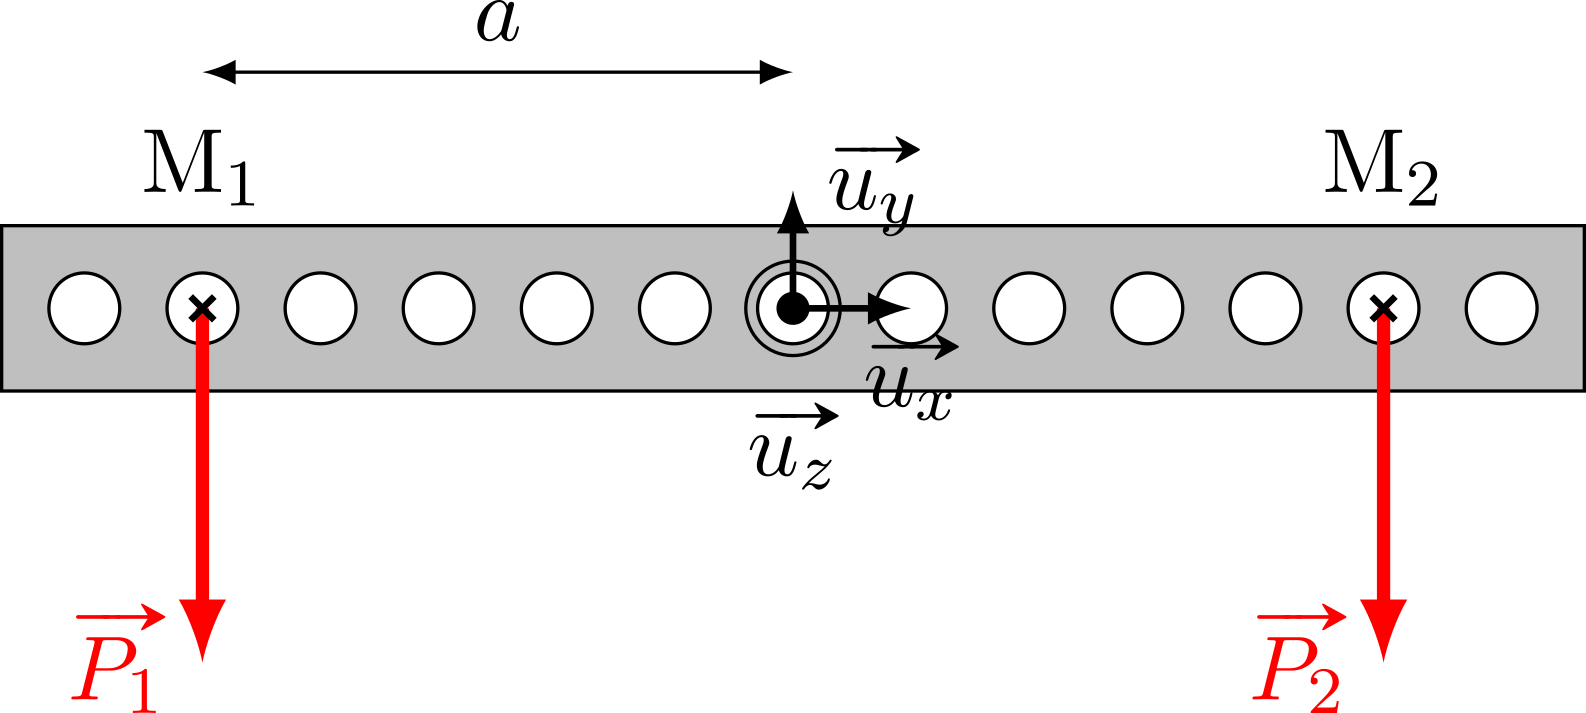
\includegraphics[scale=1]{moment_regle-a}
    \end{center}
\end{minipage}
\hfill
\begin{minipage}{0.65\linewidth}
    \begin{gather*}
        \Pf_1 = -mg\uy
        \qqet
        \OM_1 = -a\ux
        \\
        \OM\wedge\Pf_1 = (-a)\times(-mg)\ux\wedge\uy = mga\uz
        \\
        \boxed{\Mc_z(\Pf_1) = mga}
        \qqet
        \boxed{\Mc_z(\Pf_2) = -mga}
    \end{gather*}
    \centering La règle ne tourne pas.
\end{minipage}

\section{Moment cinétique}
Comme pour le chapitre de mécanique énergétique, on a commencé par introduire le
concept de travail d'une force avant de l'appliquer sous une certaine forme à
l'énergie cinétique du corps. Ici, on a défini le moment d'une force,
caractérisant sa capacité à faire tourner un point~: il paraît donc naturel de
définir une grandeur vectorielle caractérisant la rotation d'un point matériel~:
c'est le \textbf{moment cinétique}.

\subsection{Moment cinétique par rapport à un point}
\begin{tdefi}{Définition~: moment cinétique par rapport à un point, heart}
    Le moment cinétique d'un point M par rapport à un point O dans le
    référentiel $\Rc$ est le \textbf{vecteur}~:
    \[
        \boxed{\Lcf_{\Or/\Rc}(\Mr) = \OM\wedge\pf_{\Mr/\Rc} = \OM\wedge
        m\vf_{\Mr/\Rc}}
        \qquad
        \text{Unité~:~}
        \si{N.m.s}
    \]
    qui traduit la «~quantité de rotation~» d'un point matériel en rotation
    autour d'un autre.
\end{tdefi}

\textbf{Interprétation}~: considérons un repère cylindrique autour de l'axe
$(\Or z)$. On a alors
\[
    \left\{
        \begin{aligned}
            \OM &= r\ur\\
            \vf &= \rp\ur + r\w\ut
        \end{aligned}
    \right.
    \quad\Ra\quad
    \Lcf_{\Or/\Rc} = (r\ur)\wedge m(\rp\ur+r\w\ut) = mr^2\w\uz
\]
Ainsi, \textbf{le moment cinétique ne conserve une information que sur la
rotation du système}. Si celui-ci est nul tout le temps, soit il n'y a pas de
mouvement, soit le vecteur vitesse et le vecteur position sont colinéaires et le
mouvement est rectiligne.

\textbf{Interprétation géométrique}~: la \textbf{direction} de $\Lcf_{\Or}$
indique la manière dont M tourne autour de O.
\begin{center}
    \begin{tabularx}{\linewidth}{YYY}
        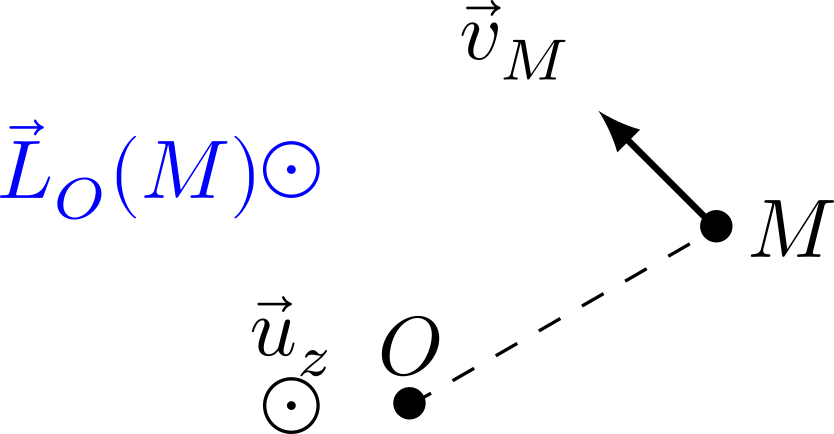
\includegraphics[scale=1]{moment_cin-a} &
        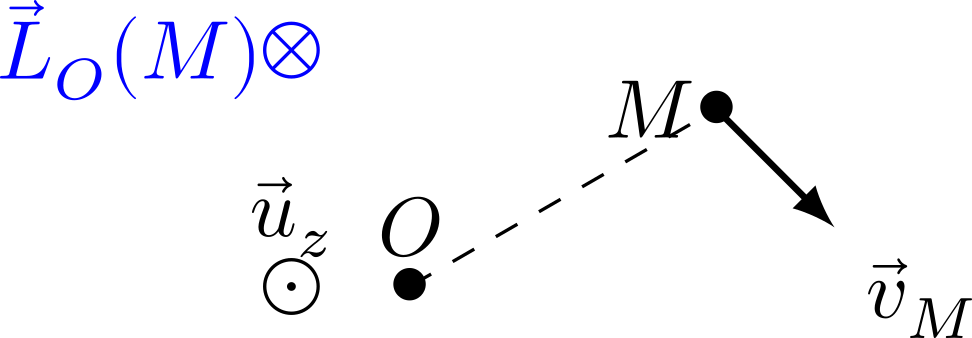
\includegraphics[scale=1]{moment_cin-b} &
        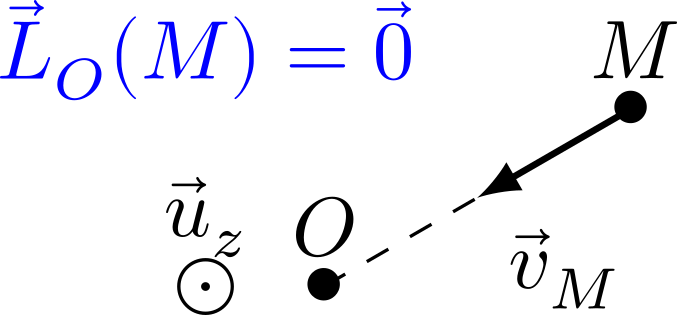
\includegraphics[scale=1]{moment_cin-c}
        \\
        Si $\Lcf_{\Or}(\Mr)$ est dirigé selon $+\uz$, M tourne autour de O dans
        le sens \textbf{direct}. &
        Si $\Lcf_{\Or}(\Mr)$ est dirigé selon $-\uz$, M tourne autour de O dans
        le sens \textbf{horaire}. &
        Si $\Lcf_{\Or}(\Mr) = \of$, M ne tourne pas autour du point O.
    \end{tabularx}
\end{center}

\begin{rimpo}{Important}
    \begin{enumerate}
        \item Le vecteur $\Lcf_{\Or}$ est orthogonal à $\OM$ et à $\vf$.
        \item Le moment cinétique $\Lcf_{\Or}$ dépend du point O~:
            \[
                \boxed{\Lcf_{\Or'}(\Mr) = \Lcf_{\Or}(\Mr) + \vv{\rm O'O}\wedge
                m\vf}
            \]
    \end{enumerate}
\end{rimpo}

\subsection{Moment cinétique par rapport à un axe \ul{orienté}}
\begin{tdefi}{Définition~: moment cinétique par rapport à un axe orienté, heart}
    Le moment cinétique d'un point M par rapport à un axe orienté $(\Or,\uz)$
    dans le référentiel $\Rc$ est le \textbf{scalaire}~:
    \[
        \boxed{\Lc_z(\Mr) = (\OM\wedge\pf_{\Mr/\Rc})\cdot\uz =
            \Lcf_{\Or/\Rc}(\Mr)\cdot\uz}
        \qquad
        \text{Unité~:~}
        \si{N.m.s}
    \]
    avec O un point de l'axe. $\Lc_z$ est donc le projeté du moment
    $\Lcf_{\Or/\Rc}$ sur $(\Or z)$.
\end{tdefi}

\textbf{Interprétation géométrique}~: cette fois-ci aussi, c'est le
\textbf{signe} de $\Lc_z$ qui indique le sens de rotation de M autour de l'axe~:
s'il est \textbf{positif} il se fait dans le sens \textbf{direct}.

\begin{rimpo}{Important}
    \begin{enumerate}
        \item $\Lc_z$ est un scalaire, alors que $\Lcf_{\Or}$ est un vecteur~!
        \item $\Lc_z$ est indépendant du point O de l'axe $(\Or z)$. En effet~:
            \[
                \Lcf_{\mathrm{O'}/\Rc}\cdot\uz =
                \left[(\vv{\rm O'O}+\OM)\wedge\pf_{\Mr/\Rc}\right]\cdot\uz =
                \underbracket[1pt]{
                (\underbracket[1pt]{\vv{\rm O'O}}_{\parr\uz}\wedge\pf_{\Mr/\Rc})
                \cdot\uz}_{=0}
                + \Lcf_{\Or/\Rc}\cdot\uz = \Lcf_{\Or/\Rc}\cdot\uz 
            \]
    \end{enumerate}
    \vspace*{-30pt}
\end{rimpo}

\section{Théorème du moment cinétique}
Rien que par les unités des différentes grandeurs, on peut imaginer le lien
entre moment cinétique et moment d'une force, ou avec un peu de recule sur ce
qu'il est en train de se passer…

\subsection{Par rapport à un point \textit{fixe}}
\begin{tprop}{Théorème du moment cinétique par rapport à un point \textit{fixe},
    heart}
    Pour un point matériel M de masse $m$ soumis à des forces extérieures
    $\Ff_i$ dans un référentiel $\Rc$ supposé galiléen et O un point
    \textbf{fixe} dans $\Rc$, on a
    \[\boxed{\dv{\Lcf_{\Or/\Rc}(\Mr)}{t} = \sum_i\Mcf_{\Or}(\Ff_i)}\]
\end{tprop}
\begin{tdemo}{Démonstration, hand}
    Comme pour un bilan de puissance où l'on applique $\cdot\vf$ sur le PFD, il
    suffit ici d'appliquer $\OM\wedge$~: \smallbreak
    \begin{side}
        On part du PFD
        \begin{align*}
            m\af &= \sum_i \Ff_i
            \\\Lra
            \dv{\pf}{t} &= \sum_i\Ff_i
            \\\Ra
            \OM\wedge\dv{\pf}{t} &= \OM\tikzmark{om}\wedge\sum_i\tikzmark{ff}\Ff_i
        \end{align*}
        \tcblower
        Or,
        \begin{align*}
            \dv{\Lcf_{\Or/\Rc}(\Mr)}{t} &= \dv{\tikzmark{dv}}{t}
                                            \left(\OM\tikzmark{omd}
                                            \wedge\pf\tikzmark{pfd}
                                            \right)
            \\
                                        &=
                                        \underbracket[1pt]{
                                            \xunderbracket{\dv{\OM}{t}}_{\parr\vf}
                                            \wedge
                                            \xunderbracket{\pf}_{\parr\vf}
                                        }_{=\of}
                                        + \OM\wedge\dv{\pf}{t}
        \end{align*}
    \end{side}
    Ainsi,
    \begin{gather*}
        \dv{\Lcf_{\Or/\Rc}(\Mr)}{t} = \sum_i\OM\wedge\Ff_i
        \Lra
        \boxed{\dv{\Lcf_{\Or/\Rc}(\Mr)}{t} = \sum_i\Mcf_{\Or}(\Ff_i)}
        \qed
    \end{gather*}
\end{tdemo}
\tikz[remember picture, overlay]
\draw[-stealth, transform canvas={yshift=12pt}]
    ([shift={(-6pt,0)}]pic cs:om) to[out=90, in=90] (pic cs:ff)
    ;
\tikz[remember picture, overlay]
\draw[-stealth, transform canvas={yshift=6pt}]
    (pic cs:dv) to[out=90, in=90] ([shift={(-6pt,6pt)}]pic cs:omd)
    ;
\tikz[remember picture, overlay]
\draw[-stealth, transform canvas={yshift=6pt}]
    (pic cs:dv) to[out=90, in=90] ([shift={(-6pt,6pt)}]pic cs:pfd)
    ;
\vspace{-20pt}

\subsection{Par rapport à un axe \ul{orienté} \textit{fixe}}
\begin{tprop}{Théorème du moment cinétique par rapport à un axe \ul{orienté}
    \textit{fixe}, heart}
    Pour un point matériel M de masse $m$ soumis à des forces extérieures
    $\Ff_i$ dans un référentiel $\Rc$ supposé galiléen et $(\Or,z)$ un axe
    orienté \textbf{fixe} dans $\Rc$, on a
    \[\boxed{\dv{\Lc_z(\Mr)}{t} = \sum_i\Mc_z(\Ff_i)}\]
\end{tprop}
\begin{tdemo}{Démonstration, hand}
    On projette simplement le TMC version vectorielle sur $\uz$~:
    \begin{align*}
        \dv{\Lcf_{\Or/\Rc}(\Mr)}{t}\cdot\uz &= \sum_i\Mcf_{\Or}(\Ff_i)\cdot\uz
        \\\Lra
        \dv{\Lcf_{\Or/\Rc}(\Mr)\cdot\uz}{t} &= \sum_i\Mc_z(\Ff_i)
        \\\Lra
        \Aboxed{\dv{\Lc_z(\Mr)}{t} &= \sum_i\Mc_z(\Ff_i)}
        \qed
    \end{align*}
\end{tdemo}

\section{Exemple du pendule simple}
\hspace*{-0.75cm}
\begin{minipage}{0.70\linewidth}
    \begin{enumerate}[label=\sqenumi]
        \litem{De quoi parle-t-on~?} On étudie le mouvement d'une masse
            suspendue à un fil, dans $\Rc\ind{laboratoire}$ supposé galiléen.
        \litem{Schéma}.
        \litem{Modélisation.} On choisit d'utiliser des coordonnées polaires.
            \begin{itemize}
                \item La masse est assimilée à un point matériel M.
                \item Origine~: point d'accroche du fil (centre de rotation
                    pendule).
                \item Repère~: $(O,\ur,\ut)$ avec base polaire (voir schéma).
                \item $t$ initial~: moment du lâché, $\tt(0) = \tt_0$ et
                    $\tt(0) = 0$.
                \item Repérage~: $\OM = \ell\ur$, $\vf = \ell\tp\ut$.
            \end{itemize}
    \end{enumerate}
\end{minipage}
\hfill
\begin{minipage}{0.25\linewidth}
    \begin{center}
        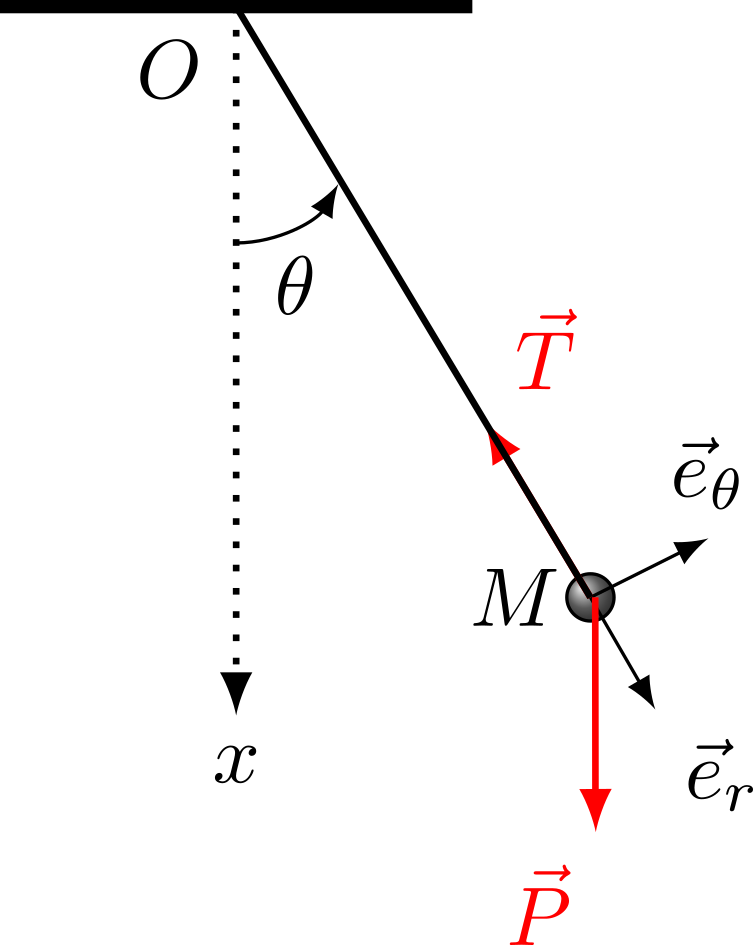
\includegraphics[width=\linewidth]{pendule_plain}
    \end{center}
\end{minipage}
\begin{enumerate}[label=\sqenumi, start=4]
    \litem{Bilan des forces.}
        \[
            \begin{array}{ll}
                \textbf{Poids} & \Pf = m\gf = mg(\cos\tt \ur - \sin\tt \ut)\\
                \textbf{Tension} & \Tf = -T\ur
            \end{array}
        \]
    \litem{Calcul des moments.}
        \[
            \left\{
                \begin{array}{rcl}
                    \Mcf_{\Or}(\Pf) & = & (\ell\ur)\wedge mg(\cos\tt \ur - \sin\tt \ut)
                                        = -mg\ell\sin\tt\uz\\
                    \Mcf_{\Or}(\Tf) & = & (\ell\ur)\wedge(-T\ur) = \of\\
                    \Lcf_{\Or}(\Mr) & = & (\ell\ur)\wedge(m\ell\tp\ut) =
                    m\ell^2\tp\uz
                \end{array}
            \right.
        \]
        Ainsi
        \[
            \boxed{\Mc_z(\Pf) = -mg\ell\sin\tt}
            \qqet
            \boxed{\Mc_z(\Tf) = 0}
            \qqet
            \boxed{\Lc_z(\Mr) = m\ell^2\tp}
        \]
    \litem{TMC}~:
    \begin{align*}
        m\ell^2\tpp &= -mg\ell\sin\tt + 0
        \\\Lra
        \Aboxed{\tpp + \frac{g}{\ell}\sin\tt &= 0}
        \qed
    \end{align*}
\end{enumerate}
On a donc bien retrouvé l'équation du mouvement du pendule simple~!

\end{document}
